\documentclass[aspectratio=169]{beamer}

\usetheme[sectionpage=none]{metropolis}

\beamertemplatenavigationsymbolsempty

\usepackage{graphicx}
\usepackage{booktabs}
\usepackage{smartdiagram}
\usepackage{minted}

\usepackage{xcolor}
\usepackage{graphicx}
\usepackage{multicol}
\usepackage{wrapfig}

\graphicspath{ {images/} }
\usepackage[export]{adjustbox}

%----------------------------------------------------------------------------------------
%	TITLE PAGE
%----------------------------------------------------------------------------------------

\title{Managing configuration drifts in large computing infrastructures:
an experimental approach at CERN}

\author{ \vspace{20px}
    \textbf{Student}: \hspace{7px} Andrea Giardini \\
    \textbf{Supervisor}: Prof. Anna Ciampolini \\
    \textbf{Mentor}: \hspace{9px} Ben Dylan Jones \\}

\institute{University of Bologna}

\date{December 19, 2016}

\begin{document}

\begin{frame}
\titlepage
\end{frame}

\begin{frame}
\frametitle{Outline}
\vspace{10px}
\tableofcontents
\end{frame}

%------------------------------------------------
%	PRESENTATION SLIDES
%------------------------------------------------

%------------------------------------------------
\section{Introduction}
%------------------------------------------------

\subsection{CERN}
\begin{frame}
    \frametitle{CERN}
    \begin{minipage}[t]{0.95\textwidth}
        \begin{columns}
            \begin{column}{0.5\textwidth}
                \begin{itemize}
                    \item European Organization for Nuclear Research
                    \item Situated in the border between Switzerland and France
                    \item 22 Member states
                    \item Big challenges
                \end{itemize}
            \end{column}
            \begin{column}{0.5\textwidth}
                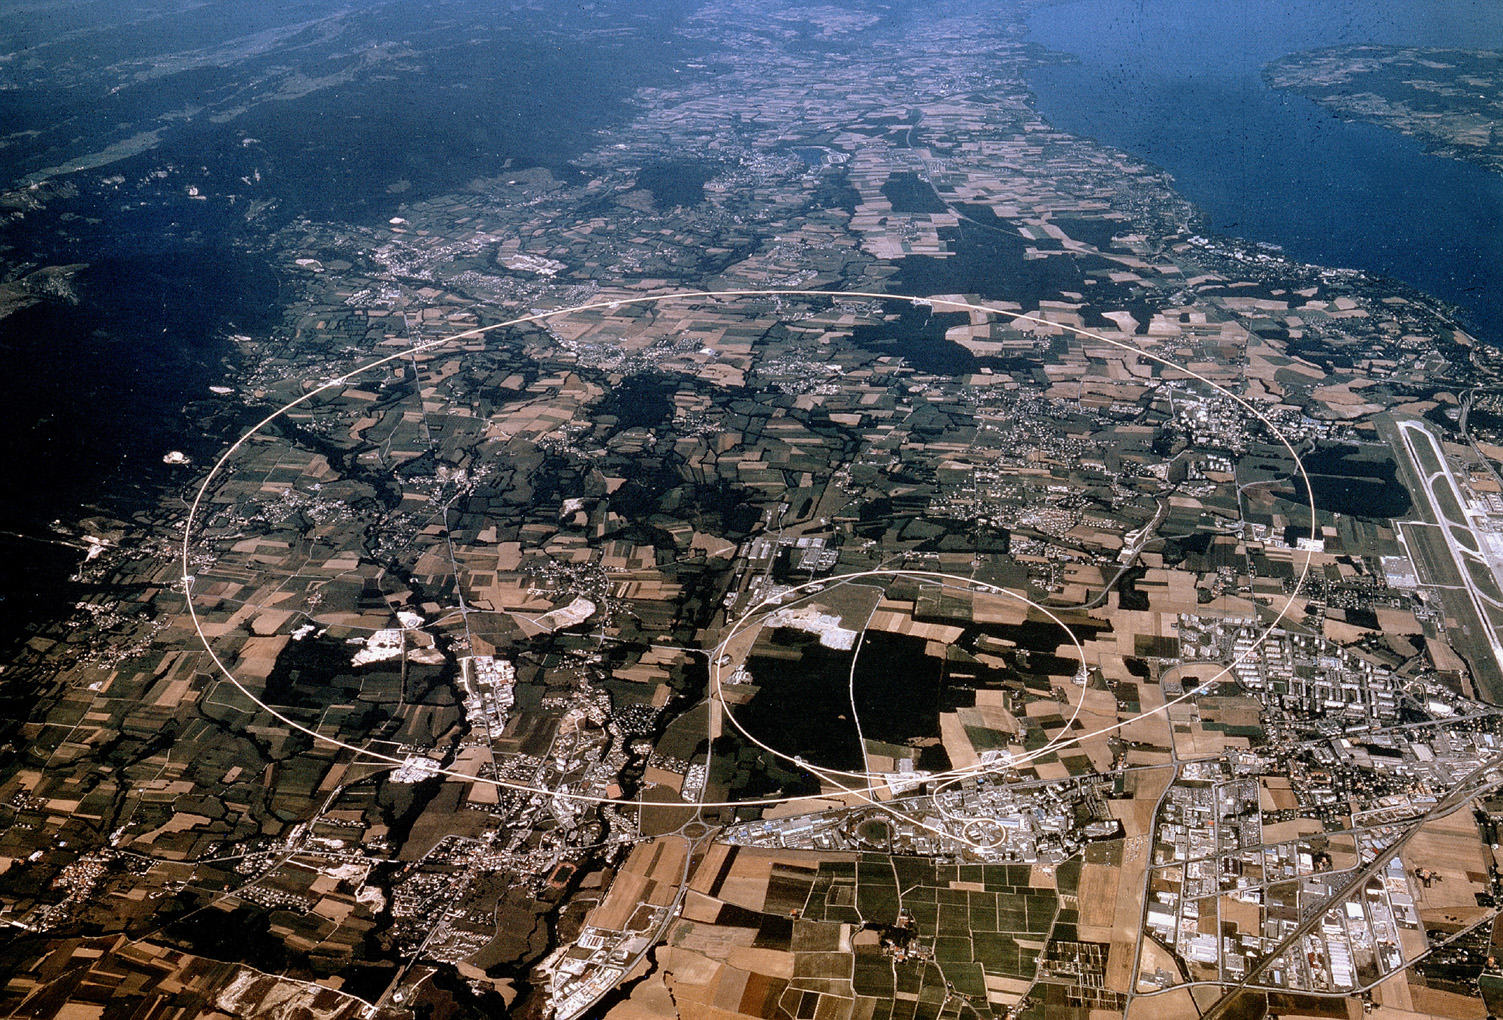
\includegraphics[width=1.1\textwidth]{CernMap.jpg}
            \end{column}
        \end{columns}
    \end{minipage}
\end{frame}

%------------------------------------------------

\begin{frame}
    \frametitle{Data Centres}
    \begin{minipage}[t]{0.95\textwidth}
        \begin{columns}[T]
            \begin{column}{0.5\textwidth}
                Two data centers:
                \begin{itemize}
                    \item Geneva
                    \item Budapest
                \end{itemize}
                Two dedicated links:
                \begin{itemize}
                    \item 2 x 100Gbps
                \end{itemize}
                \vspace{0.1in}
                The number of resources is growing year by year.
                As today:
                \begin{itemize}
                    \item 18k servers
                    \item 180PB on tape
                    \item 260PB on disk
                \end{itemize}
            \end{column}
            \begin{column}{0.5\textwidth}
                \vspace{0.5in}
                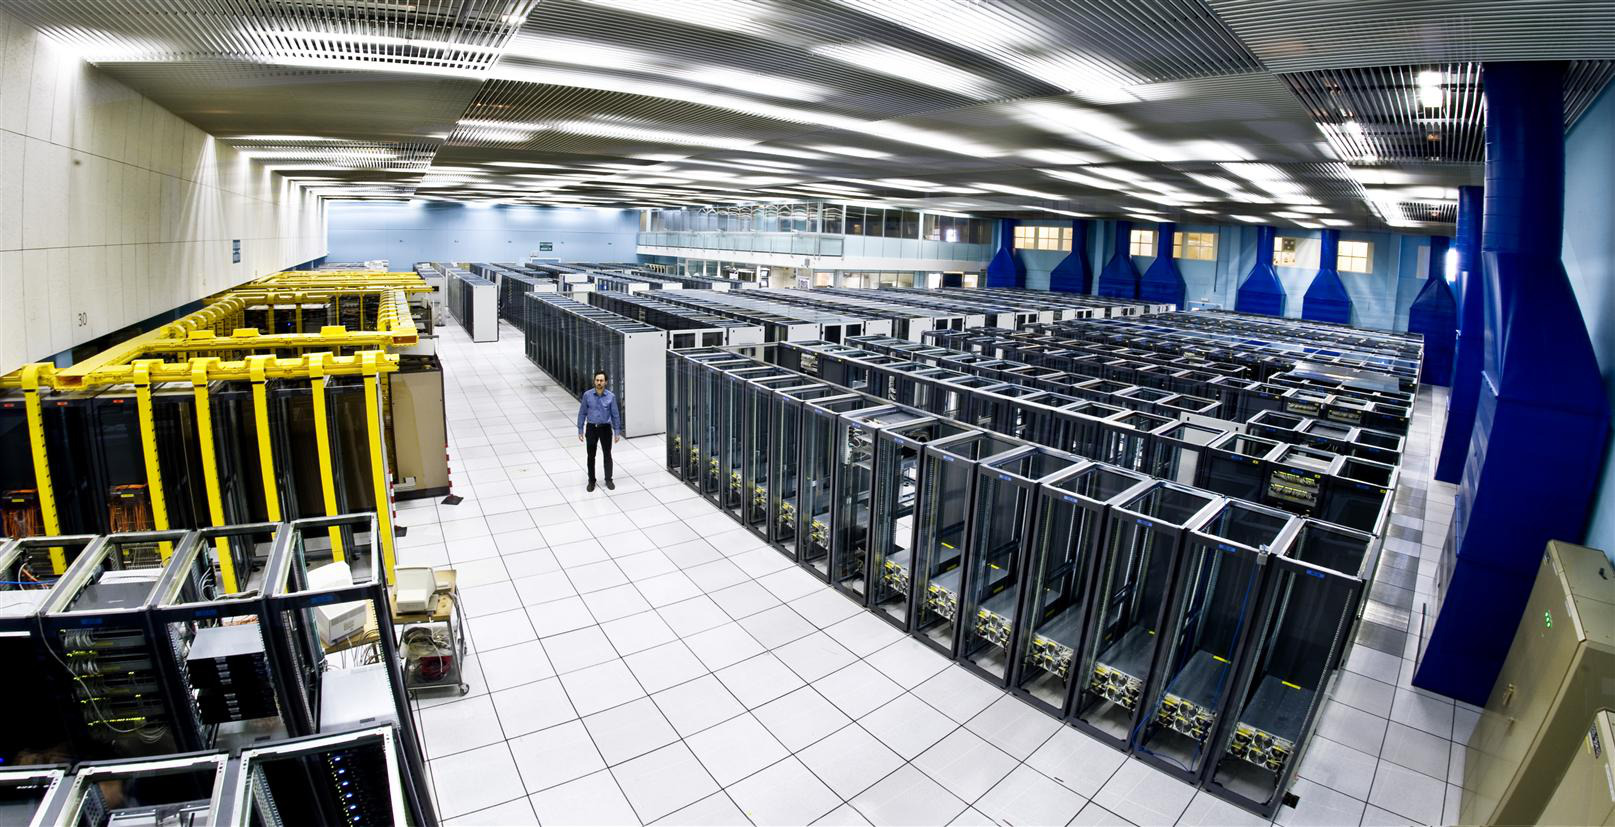
\includegraphics[width=1.1\textwidth]{DC_overview.png}
            \end{column}
        \end{columns}
    \end{minipage}
\end{frame}

%------------------------------------------------

\subsection{Configuration management}
\begin{frame}
    \frametitle{Cloud Computing}
    \begin{minipage}[t]{0.95\textwidth}
        \begin{columns}
            \begin{column}{0.8\textwidth}
                Requirements started to grow
                \begin{itemize}
                    \item Agile approach was needed
                \end{itemize}
                Since a few years we started using \textbf{Openstack} to
                deploy virtual machines for our users and Puppet to
                configure the services
            \end{column}
            \begin{column}{0.2\textwidth}
                
\includegraphics[width=0.9\textwidth]{openstack-logo512.png}
            \end{column}
        \end{columns}
    \end{minipage}
    \vspace{\belowdisplayskip}
    \vspace{\belowdisplayskip}
    \begin{minipage}[t]{0.95\textwidth}
        \begin{center}
        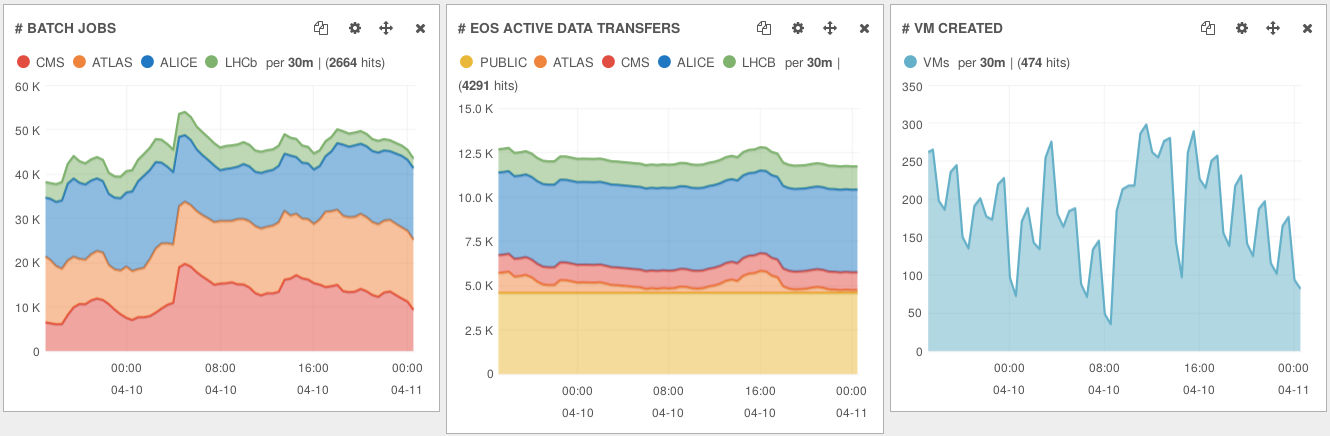
\includegraphics[width=0.83\textwidth]{Eos-CreatedVm.png}
    \end{center}
    \end{minipage}
\end{frame}

%------------------------------------------------

\begin{frame}
    \frametitle{Configuration Management with Puppet}
    \begin{minipage}[t]{0.95\textwidth}
        \begin{columns}
            \begin{column}{0.5\textwidth}
                \textbf{Puppet} is an open-source \textbf{configuration management tool}.
                It is designed to manage the configuration of Unix-like and Microsoft Windows systems declaratively. \\
                \begin{itemize}
                    \item Service configuration
                    \item Users/Groups management
                    \item Automates repetitive tasks
                \end{itemize}
            \end{column}
            \begin{column}{0.5\textwidth}
                \vspace{-10px}
                
\includegraphics[width=1.1\textwidth]{puppet-labs-logo.png}
            \end{column}
        \end{columns}
    \end{minipage}
\end{frame}

%------------------------------------------------
\section{Package Inventory}
%------------------------------------------------

\begin{frame}
    \frametitle{Package Inventory - Introduction}
    \vspace{10px}
    \begin{minipage}[t]{0.95\textwidth}
        \textbf{Package drifts} started to be a problem:
        \begin{itemize}
            \item Servers with outdated packages
            \item Difficult to spot
            \item Users forcing their servers not to update
        \end{itemize}
        It is not easy to keep all the packages in sync and guarantee security
    \end{minipage}
    \vspace{\belowdisplayskip}
    \begin{minipage}[t]{0.95\textwidth}
        \begin{center}
            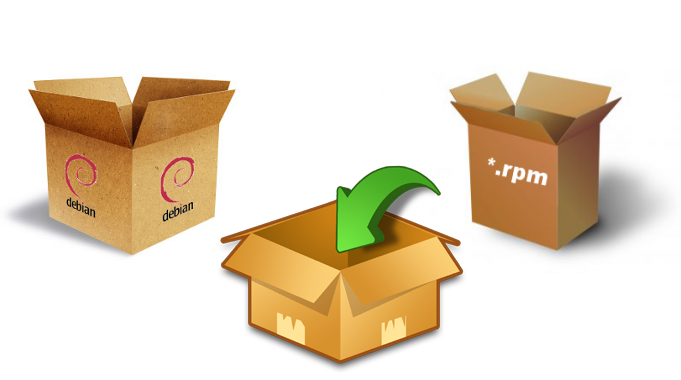
\includegraphics[width=0.5\textwidth]{package.png}
        \end{center}
    \end{minipage}
\end{frame}

%------------------------------------------------

\subsection{Project Structure}
\begin{frame}
    \frametitle{Package Inventory - Project Structure}
    The configuration team needed a tool to query packages over a large
    number of hosts in a timely manner.

    \textbf{Package Inventory} is made by three components:
    \begin{itemize}
        \item Reporter
        \item Elasticsearch Cluster
        \item Cli (Command-line Interface)
    \end{itemize}
\end{frame}

%------------------------------------------------

\begin{frame}
    \frametitle{Package Inventory - Reporter}

    Software installed on every server, integrated with Yum using a plugin.

    \begin{itemize}
        \item Reports to Elasticsearch every package change
        \item Fault-tolerant
        \item Real-time updates
    \end{itemize}

    Elasticsearch stores and indexes all the metrics to make them searchable.

    \begin{center}
        \vspace{10px}
        \smartdiagramset{sequence item border color=black,
            sequence item border size=1pt,
            sequence item font size=\small\sffamily,
            set color list={green!50,green!50,green!50}
        }
        \smartdiagram[sequence diagram]
            {Change on package status,
            Reporter collects the changes,
            Sends new metrics to Elasticsearch}
    \end{center}
\end{frame}

%------------------------------------------------

\begin{frame}[fragile]
    \frametitle{Package Inventory - Command-line Interface}
    \begin{minipage}[t]{0.95\textwidth}
        \begin{columns}
        \begin{column}{0.5\textwidth}
            The \textbf{Cli} is used by the users to query the metrics that are
            stored in the  Elasticsearch cluster.

            \begin{itemize}
                \item Possibility to compare clusters of machines
                \item Package history
                \item Package version across a set of servers
            \end{itemize}

            \textbf{Optimized to scale for large queries}:
            Query time to compare over twenty hundreds hosts is two minutes.
        \end{column}
        \begin{column}{0.5\textwidth}
            \linespread{1px}
            \begin{minted}[fontsize=\footnotesize]{bash}
pkginv -H bi/batch/gridworker/aishare
       -e production
       compare

Processing hosts with:

  - Hostgroup: bi/batch/gridworker/aishare
  - Environment: production

+------------+------------+------------+
|  Group 0   |  Group 1   |  Group 2   |
+------------+------------+------------+
| b6b3d71dfa | b6b1576a51 | b60ba703db |
| b636f67ca8 | b604a66b3b | b6e493a1b6 |
| b62b21e394 | b6c6f66a36 |            |
| b65573753a | b67d439ea5 |            |
| b6a09855b8 |            |            |
| b6a2bb83c8 |            |            |
| b67af0481a |            |            |
| b64f0f53c1 |            |            |
| b69b92afd1 |            |            |
| b67f818ae3 |            |            |
| b67cc79825 |            |            |
| b622b1cfdc |            |            |
+------------+------------+------------+
            \end{minted}
        \end{column}
        \end{columns}
    \end{minipage}
\end{frame}

%------------------------------------------------

\begin{frame}[fragile]
    \frametitle{Package Inventory - Command-line Interface}
    \begin{minipage}[t]{0.95\textwidth}

        Now that we know which hosts are drifting we can get more details.

        Packages can have:
        \begin{itemize}
            \item Different versions
            \item Different status
        \end{itemize}

        Comparing two hosts gives us details about the installed packages.
        \vspace{10px}
    \end{minipage}
    \vspace{\belowdisplayskip}
    \begin{minipage}[t]{0.95\textwidth}
        \centering
        \linespread{1px}
        \begin{minted}[fontsize=\footnotesize]{bash}
               pkginv -m 'b6b3d71dfa b6b1576a51' compare

               +--------------------+-------+------------+-------------+
               |       Package      | Field | b6b3d71dfa |  b6b1576a51 |
               +--------------------+-------+------------+-------------+
               |       httpd        |       |  Present   | Not present |
               |    httpd-tools     |       |  Present   | Not present |
               |      gridsite      |       |  Present   | Not present |
               |      mod_ssl       |       |  Present   | Not present |
               |     castor-lib     | epoch |   8.slc6   |    9.slc6   |
               | castor-rfio-client | epoch |   8.slc6   |    9.slc6   |
               |  castor-ns-client  | epoch |   8.slc6   |    9.slc6   |
               |    castor-devel    | epoch |   8.slc6   |    9.slc6   |
               +--------------------+-------+------------+-------------+
        \end{minted}
    \end{minipage}
\end{frame}

%------------------------------------------------

\subsection{Results}
\begin{frame}
    \frametitle{Package Inventory - Results}
    \begin{itemize}
        \item Installed in more than \textbf{55 hundreds of servers}
        \item Spotted over \textbf{two hundreds of servers} out of sync
        \item Used extensively to monitor the deployment of security updates
        \item Debugging performance issues
    \end{itemize}
\end{frame}

%------------------------------------------------
\section{Continuous Integration}
%------------------------------------------------

\begin{frame}
    \frametitle{Continuous Integration - Introduction}
    Shipping changes to production used to be a manual procedure:
    \begin{itemize}
        \item Multiple actions involved
        \item Human error
    \end{itemize}

    The process can be automated:
    \begin{itemize}
        \item Less time wasted
        \item More organization
    \end{itemize}
\end{frame}

%------------------------------------------------

\subsection{Project Structure}
\begin{frame}
    \frametitle{Continuous Integration - Project Structure}
    \begin{minipage}[t]{0.95\textwidth}
        \begin{columns}
            \begin{column}{0.5\textwidth}
            Implementation of a Continuous Integration platform using \textbf{Jenkins}
            \begin{itemize}
                \item Open source software
                \item Highly customizable
                \item Active community
            \end{itemize}
            \end{column}
            \begin{column}{0.5\textwidth}
                \vspace{-10px}
                
\includegraphics[width=1.1\textwidth]{jenkins-logo.png}
            \end{column}
        \end{columns}
    \end{minipage}
\end{frame}

%------------------------------------------------

\begin{frame}
    \frametitle{Manual configuration change process}
    \smartdiagramset{sequence item border color=black,
        sequence item border size=1pt,
        sequence item font size=\small\sffamily,
        set color list={red!50,red!50,red!50}
    }
    \smartdiagram[sequence diagram]
        {Push the change to custom Git branch,
        Open JIRA issue describing the change,
        Open merge request on Gitlab to QA}
    \vspace{20px}
    \smartdiagram[sequence diagram]
        {Approve merge request on Gitlab,
        Open merge request on Gitlab to master,
        Approve merge request on Gitlab}
\end{frame}

%------------------------------------------------

\begin{frame}
    \frametitle{Automated configuration change process}
    \smartdiagramset{sequence item border color=black,
        sequence item border size=1pt,
        sequence item font size=\small\sffamily,
        set color list={red!50,red!50,orange!50}
    }
    \smartdiagram[sequence diagram]
        {Push the change to custom Git branch,
        Open JIRA issue describing the change,
        Open merge request on Gitlab to QA}
    \vspace{20px}
    \smartdiagramset{set color list={red!50,red!50,red!50}}
    \smartdiagram[sequence diagram]
        {Approve merge request on Gitlab,
        Open merge request on Gitlab to master,
        Approve merge request on Gitlab}
\end{frame}

%------------------------------------------------

\begin{frame}
    \frametitle{Automated configuration change process}
    \smartdiagramset{sequence item border color=black,
        sequence item border size=1pt,
        sequence item font size=\small\sffamily,
        set color list={red!50,red!50,orange!50,green!50}
    }
    \smartdiagram[sequence diagram]
        {Push the change to custom Git branch,
        Open JIRA issue describing the change,
        Open merge request on Gitlab to QA,
        Run automated tests on Jenkins}
    \vspace{20px}
    \smartdiagramset{set color list={red!50,red!50,red!50}}
    \smartdiagram[sequence diagram]
        {Approve merge request on Gitlab,
        Open merge request on Gitlab to master,
        Approve merge request on Gitlab}
\end{frame}

%------------------------------------------------

\begin{frame}
    \frametitle{Automated configuration change process}
    \smartdiagramset{sequence item border color=black,
        sequence item border size=1pt,
        sequence item font size=\small\sffamily,
        set color list={red!50,red!50,orange!50,green!50}
    }
    \smartdiagram[sequence diagram]
        {Push the change to custom Git branch,
        Open JIRA issue describing the change,
        Open merge request on Gitlab to QA,
        Run automated tests on Jenkins}
    \vspace{20px}
    \smartdiagramset{set color list={orange!50,red!50,red!50}}
    \smartdiagram[sequence diagram]
        {Approve merge request on Gitlab,
        Open merge request on Gitlab to master,
        Approve merge request on Gitlab}
\end{frame}

%------------------------------------------------

\begin{frame}
    \frametitle{Automated configuration change process}
    \smartdiagramset{sequence item border color=black,
        sequence item border size=1pt,
        sequence item font size=\small\sffamily,
        set color list={red!50,red!50,orange!50,green!50}
    }
    \smartdiagram[sequence diagram]
        {Push the change to custom Git branch,
        Open JIRA issue describing the change,
        Open merge request on Gitlab to QA,
        Run automated tests on Jenkins}
    \vspace{20px}
    \smartdiagramset{set color list={orange!50,orange!50,red!50}}
    \smartdiagram[sequence diagram]
        {Approve merge request on Gitlab,
        Open merge request on Gitlab to master,
        Approve merge request on Gitlab}
\end{frame}

%------------------------------------------------

\begin{frame}
    \frametitle{Automated configuration change process}
    \smartdiagramset{sequence item border color=black,
        sequence item border size=1pt,
        sequence item font size=\small\sffamily,
        set color list={red!50,red!50,orange!50,green!50}
    }
    \smartdiagram[sequence diagram]
        {Push the change to custom Git branch,
        Open JIRA issue describing the change,
        Open merge request on Gitlab to QA,
        Run automated tests on Jenkins}
    \vspace{20px}
    \smartdiagramset{set color list={orange!50,orange!50,green!50,red!50}}
    \smartdiagram[sequence diagram]
        {Approve merge request on Gitlab,
        Open merge request on Gitlab to master,
        Run automated tests on Jenkins,
        Approve merge request on Gitlab}
\end{frame}

%------------------------------------------------

\begin{frame}
    \frametitle{Automated configuration change process}
    \smartdiagramset{sequence item border color=black,
        sequence item border size=1pt,
        sequence item font size=\small\sffamily,
        set color list={red!50,red!50,orange!50,green!50}
    }
    \smartdiagram[sequence diagram]
        {Push the change to custom Git branch,
        Open JIRA issue describing the change,
        Open merge request on Gitlab to QA,
        Run automated tests on Jenkins}
    \vspace{20px}
    \smartdiagramset{set color list={orange!50,orange!50,green!50,orange!50}}
    \smartdiagram[sequence diagram]
        {Approve merge request on Gitlab,
        Open merge request on Gitlab to master,
        Run automated tests on Jenkins,
        Approve merge request on Gitlab}
\end{frame}

%------------------------------------------------

\begin{frame}
    \frametitle{Gitlab merge request}
    \centering
    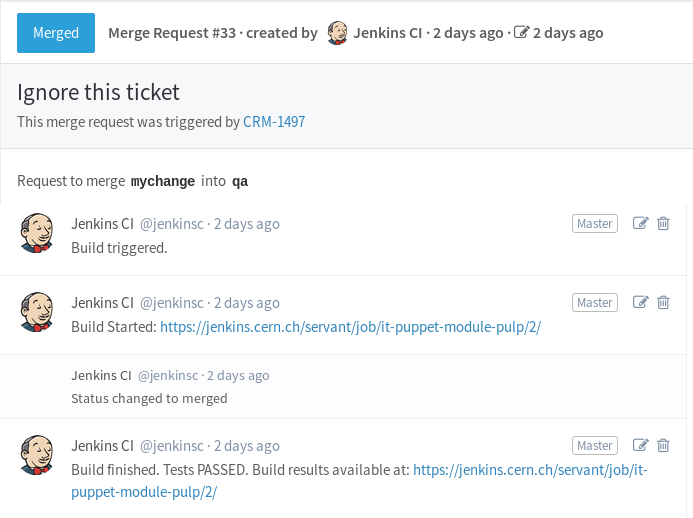
\includegraphics[width=0.7\textwidth]{gitlab_merge_to_qa_final.jpg}
\end{frame}

%------------------------------------------------

\subsection{Results}
\begin{frame}
    \frametitle{Continuous Integration - Results}
    \begin{itemize}
        \item \textbf{Extremely customizable infrastructure}
        \begin{itemize}
            \item Users can define their tests
            \item Service managers specify how the test server needs to be built
            \item Tests can be re-triggered with a comment on GitLab or pushing new commits
        \end{itemize}
        \item \textbf{Procedure completely automated}
        \item Every service manager is responsible for its Puppet module
        \item No need for users to learn how to use Jenkins
    \end{itemize}
\end{frame}

%------------------------------------------------
\section{Conclusions}
%------------------------------------------------

\begin{frame}
    \frametitle{Conclusions}

    \textbf{Package Inventory} and the \textbf{Continuous integration}
    platform have been \textbf{successfully integrated in the
    infrastructure at CERN}.

    Package Inventory has been used to spot several inconsistency and it has
    been used extensively to report several misconfigurations.

    The Continuous Integration platform has been used to automate the
    deployment of changes to production. Unfortunately, writing meaningful
    tests requires effort: obtaining a fully automated pipeline with complete
    tests will require time.
\end{frame}

%------------------------------------------------

\begin{frame}
    \frametitle{Questions}

\begin{center}
\Huge Questions ?
\end{center}
\end{frame}
\end{document}
